\section*{\code{phd-tester}}

\begin{frame}{Main Ideas}
    \begin{block}{\phantom{}}
    Each \textbf{test} $t \in \mathcal{T}$ involves a \textbf{stuff} $s \in \mathcal{S}$ to test (\eg{} algorithm) and an \textbf{environment} $e \in \mathcal{E}$ where the test occurs (\eg{} path finding map) Each \textbf{stuff}(\textbf{environment}) is a tuple of $n$($m$) values of parameters $p_i \in \mathcal{P}$ (\eg{} number of edge to perturbate, heuristic to use), where each parameter value $v_i$ has a specific domain $\mathcal{D}_{i} \cup \{nil \}$ (NIL). All Elements in $\mathcal{S}$($\mathcal{E}$) share the same tuple structure.
    \end{block}
    \vspace{-5pt}
    \begin{block}{\phantom{}}
        The final application is composed by 2 parts:
        \begin{enumerate}
            \item a \textbf{library} which the user call and provide a \textit{template design pattern} with easy APIs (provided by \code{phd-tester});
            \item a \textbf{user code} which implements the \textit{template design pattern}, providing mandatory information about the test as well as actually call the program to test (pro: test can be coded with any language!).
        \end{enumerate}
    \end{block}
    
\end{frame}

\begin{frame}{Template to follow}
    High-level steps in the \textit{template} provided by the framework:
    \begin{enumerate}
        \item the user specifies all the parameter values he wants (\eg{} perturbation generation policy $\in \{ \mbox{random}, \mbox{area} \}$);
        \item the application generates all the required tests $\mathcal{T}^{*} \subseteq \mathcal{T}$;
        \item the application executes all the tests $t \in \mathcal{T}^{*}$;
        \item the application produces generate $n$ CSVs representing test outcome (note $n \geq |\mathcal{T}^{*}|$);
    \end{enumerate}
\end{frame}

\begin{frame}{Option Graph}
    \begin{block}{\hphantom{}}
        The user specifies all the parameter values he wants (\eg{} perturbation generation policy $\in \{ \mbox{random}, \mbox{area} \}$);
    \end{block}

    \begin{minipage}{0.49\textwidth}
        By command line. In order to build the CLI interface, developer needs in \textit{user code} to declare the \textbf{option graph}: $\forall p_i \in \mathcal{P}$ say its domain $\mathcal{D}_i$, and what constraints it implies (\eg{} if parameter \code{perturbationPolicy} is set to \code{random}, then the CLI needs to specify parameter value \code{edge number}).
    \end{minipage}\hfill%
    \begin{minipage}{0.49\textwidth}
        \begin{tikzpicture}
            \tikzstyle{vertex} = [shape=rectangle, rounded corners=1mm, draw=blue!50, fill=blue!20, thick, minimum size=3mm, inner sep=3pt, node distance=1.0cm and 0.1cm];
\tikzstyle{vertex2} = [shape=rectangle, rounded corners=1mm, draw=red!50, fill=red!20, thick, minimum size=3mm, inner sep=3pt, node distance=1cm and 0.1cm];
\tikzstyle{vertex3} = [shape=rectangle, rounded corners=1mm, draw=green!50, fill=green!20, thick, minimum size=3mm, inner sep=3pt, node distance=1cm and 0.1cm];
\tikzstyle{vertex4} = [shape=rectangle, rounded corners=1mm, draw=yellow!50, fill=yellow!20, thick, minimum size=3mm, inner sep=3pt, node distance=1cm and 0.1cm];
\tikzstyle{vertex5} = [shape=rectangle, rounded corners=1mm, draw=cyan!50, fill=cyan!20, thick, minimum size=3mm, inner sep=3pt, node distance=1cm and 0.1cm];

\node[vertex3](Maps) at (0,0) {Maps};
\node[vertex, right=of Maps](Perturbations) {Perturbations};
\node[vertex, below =of Perturbations](Random) {Random};
\node[vertex, left =of Random](Area) {Area};
\node[vertex2, below right =of Random](Edges) {\# Edges};
\node[vertex4, below left =of Area](Radius) {Radius};
\node[vertex5, below right=of Area](Location) {Location};

\draw[-{Latex[length=2mm,width=3mm]}, line width=1mm]
    (Perturbations) edge node[]{} (Random) 
    (Perturbations) edge node[]{} (Area) 
    (Random) edge node[]{} (Edges) 
    (Area) edge node[]{} (Radius)
    (Area) edge node[]{} (Location)  
;
        \end{tikzpicture}
    \end{minipage}
\end{frame}

\begin{frame}{Example of Option graph}
    \begin{figure}
        \begin{subfigure}{1.0\textwidth}
            \centering
            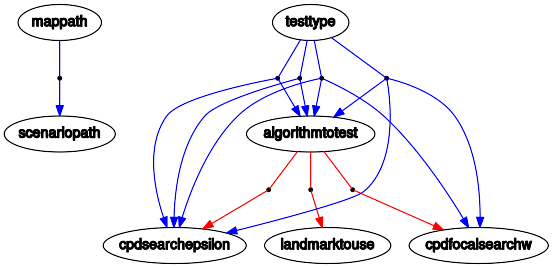
\includegraphics[width=0.9\textwidth]{src/images/optionGraph1.png}
        \end{subfigure}\\
        \begin{subfigure}{1.0\textwidth}
            \centering
            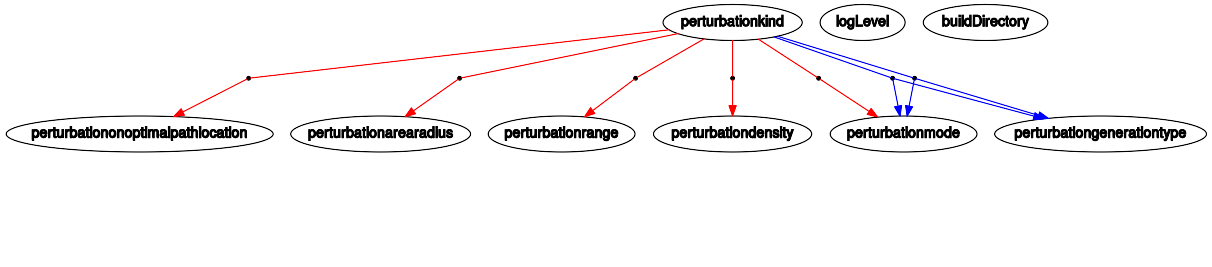
\includegraphics[width=1.09\textwidth]{src/images/optionGraph2.png}
        \end{subfigure}
    \end{figure}
\end{frame}

\begin{frame}{CLI generated}
    \begin{figure}
        \centering
        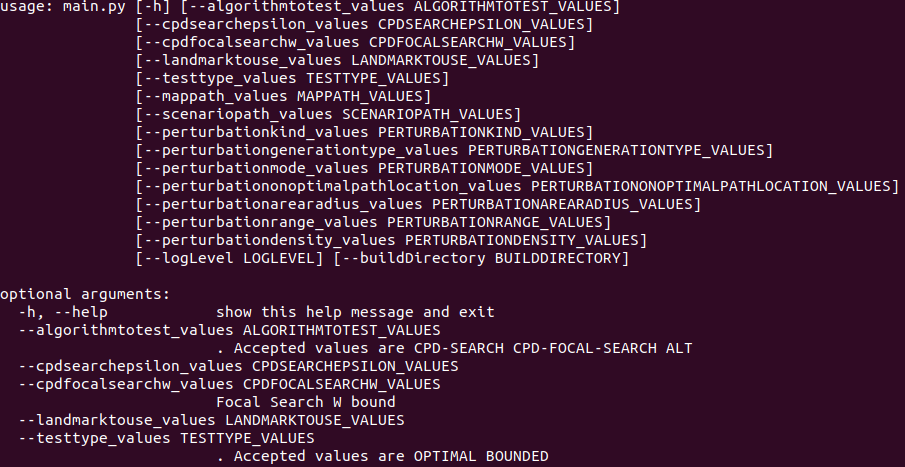
\includegraphics[width=1.0\textwidth]{src/images/help.png}
    \end{figure}
\end{frame}

\begin{frame}{Generation of $\mathcal{T}^{*}$}
    \begin{block}{\hphantom{}}
        the application generates all the required tests $\mathcal{T}^{*} \subseteq \mathcal{T}$.
    \end{block}

    $\mathcal{T}^{*}$ represents all the tests which we are required to execute. Some cartesian products in $\mathcal{S} \times \mathcal{E}$ are simply invalid (\eg{} \code{number of edges} to perturbate set to $\squote{nil}$ when the \code{perturbation policy} is $random$).

    \code{phd-tester} exploits the option graph not only to generate the CLI, but also to detect parameters dependencies.
    
    \textbf{Example:} Given a $t \in \mathcal{T}$ if \code{perturbation policy} is $random$, require that \code{number of edges}$\not = \squote{nil}$: if it is true, add $t$ in $\mathcal{T}^{*}$).
\end{frame}

\begin{frame}{Execute tests}

    \begin{block}{\hphantom{}}
        The application produces generate $n$ CSVs representing test outcome (note $n \geq |\mathcal{T}^{*}|$);
    \end{block}

    In this step the \textbf{user code} has all the freedom it desires. Usually the developer is expected to call an external program (\eg{} coded in \code{C} or in \code{C++}) that actually performs the test. As a side effect, one or more CSVs are expected to be produced somewhere (\ie{} file system, ArangoDB, mySQL $\Rightarrow$ \textbf{Data source}).

    \begin{itemize}
        \item \textbf{Problem:} how to identify which CSVs have been generated by which test $t \in \mathcal{T}^{*}$?
        \item \textbf{Solution:} by creating a new naming convention of file: \code{KS001};
    \end{itemize}
\end{frame}

\begin{frame}{\code{KS001} standard}
    \vspace{-9pt}
    \begin{block}{Idea}
        The filename is composed by \code{basename} and \code{extension}. \code{basename} is a \textbf{ordered} sequence of substring separated by \code{|}, and it is optionally prefixed by a \code{label}. Each substring is a unordered sequence of keyvalues string, separated by \code{\_}. Each keyvalue follows the pattern \code{key=value}.
    \end{block}
    \vspace{-3pt}
    \begin{figure}[h]
        \centering
        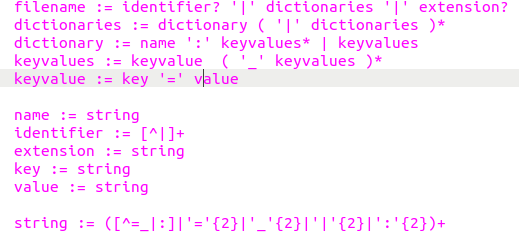
\includegraphics[width=1.0\textwidth]{src/images/ks001.png}
    \end{figure}
\end{frame}

\begin{frame}{Example of \code{KS001}}
    
    \begin{block}{\hphantom{}}
        \code{%
            |{\color{red}mp}=16room\_\_003.map\_pd=0.1\_pgt=PER-SCENARIO\_pk=RANDOM
            \_pm=MULTIPLY\_pr=[3,3]\_sp={\color{blue!50!green!50}16room\_\_003.map.scen}
            |{\color{blue}generated}:type=id-over-time|{\color{orange}.csv}
        }
    \end{block}

    \begin{itemize}
        \item doubling special characters if shown in key(value);
        \item aliasing of key(values) to avoid long names (you may reach path size limit);
        \item labelling of dictionary increase readability;
        \item \code{phd-tester} offers a set of function to query and manage \code{KS001} compliant strings;
    \end{itemize}
    
\end{frame}

\begin{frame}{Generation of interesting data (1)}
    \begin{block}{\hphantom{}}
        The application produces generate $n$ CSVs representing test outcome (note $n \geq |\mathcal{T}^{*}|$);
    \end{block}

    We use all the CSVs produced in the previous phase and stored in a \textbf{data source} to generate \textit{new} CSVs representing the benchmarks (and optionally, the related graphs as well).

    \begin{figure}
        \centering
        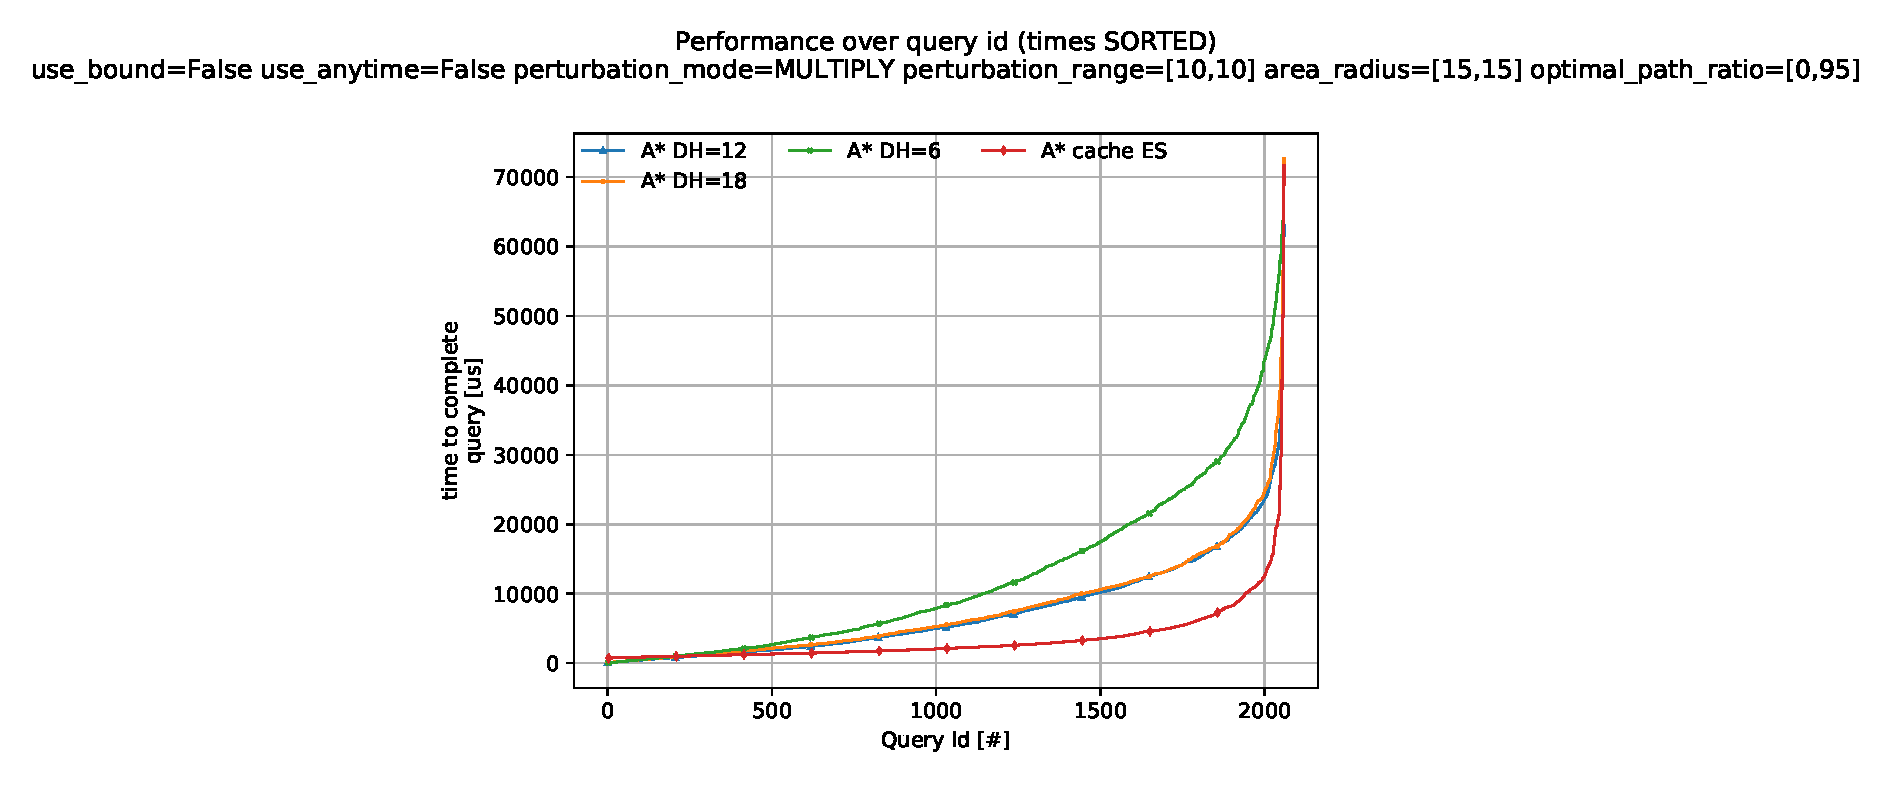
\includegraphics[width=1.0\textwidth]{src/images/example.eps}
    \end{figure}
\end{frame}

\begin{frame}{Generation of interesting data (2)}
    \code{phd-tester} dynamically generate these csv(image).

    \begin{itemize}
        \item each csv(image) is often produced by analyzing one or more outputs of tests in $\mathcal{T}^{*}$;
        \item \code{phd-tester} provides \textbf{masks}, which acts as filter allowing the software to fetch a subset of $\mathcal{T}^{*}$ to consider to produce a new csv(image) (\eg{} produce time used by all algorithm depending on the number of edge perturbated in the map);
        \item The number of CSVs to analyze may be huge (maybe over 30000, each with 100 an more rows!). \code{phd-tester} used \code{pandas} along with \code{dask} to concurrently computes the operations $\Rightarrow$ fast;
        \item \code{CurveChanger}: allows to further alters the functions generated by adding/removing/sorting values;
    \end{itemize}
\end{frame}


